\section{Andmejälgija} \label{Andmejälgija}

\subsection{The protocol} \label{protocol_desc}

Andmejälgija is a protocol that state databases are responsible for implementing themselves. In order for the database to offer an Andmejälgija service, they have to create an X-Road interface according to RIA specification\footnote{\url{https://github.com/e-gov/AJ/blob/master/doc/spetsifikatsioonid/Kasutusteabe_esitamise_protokoll.md}}. 

X-Road is a REST-based protocol which is used for secure data exchange between Estonian information systems over the Internet.

The Andmejälgija X-Road interface is expected to have the following endpoints:

\textbf{findUsage}

A query searches the data recorder database for usage records that match the constraints given in the input. The output of the query returns all records found.\cite{aj-github-spec}

\textbf{usagePeriod}

The time period for which usage information can be requested.\cite{aj-github-spec}

\textbf{heartbeat}

Requesting the availability status of the tracker's usage information.\cite{aj-github-spec}


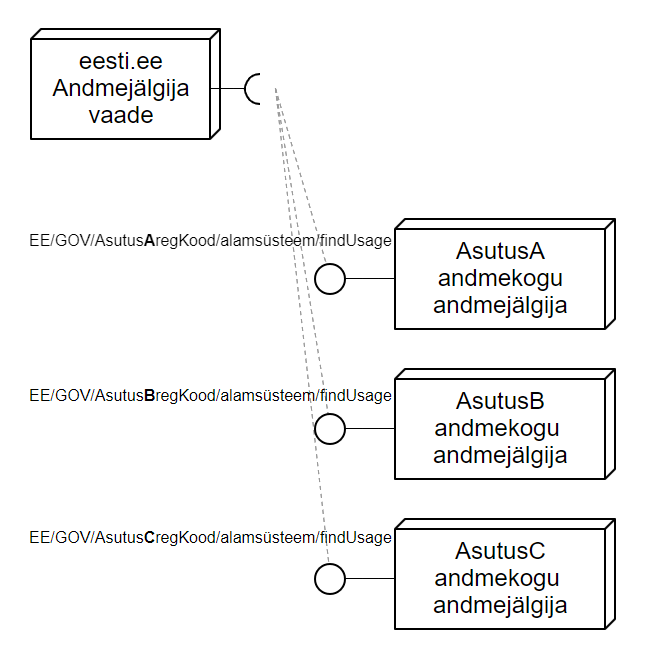
\includegraphics[width=450px]{english/figures/aj_model.PNG}

\subsection{Usage}
There are several ways for end-users to access their Data Tracker data. State portal eesti.ee provides a web-view for Andmejälgija where end users can access their data access logs. Recently, RIA have also published a mobile app for eesti.ee, that also features a view of data access logs. 

Another way to access Andmejälgija data is through Rahvastikuregister, although, for some reason, not all state databases that are covered by Eesti.ee are covered by Rahvastikuregister.



\subsection{Adoption}
The current adoption of Andmejälgija is flawed, to say the least. Very often it is not at all clear why your data have been accessed, at least from the first glance. Explanation messages are vague and confusing, often being similar to "data access by personal code", making it difficult to understand the reason behind the data access, even if it was you who accessed it.

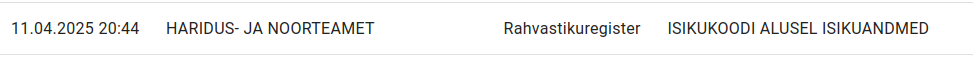
\includegraphics[width=450px]{english/figures/bad_aj_desc.png}

There is even an information sheet with recommendations for services implementing the Andmejälgija protocol, and it states that providing poor quality explanations for data access is a bad practice.\footnote{\url{https://www.ria.ee/sites/default/files/documents/2022-11/Soovitusi-Andmejalgija-rakendamiseks.pdf}} 

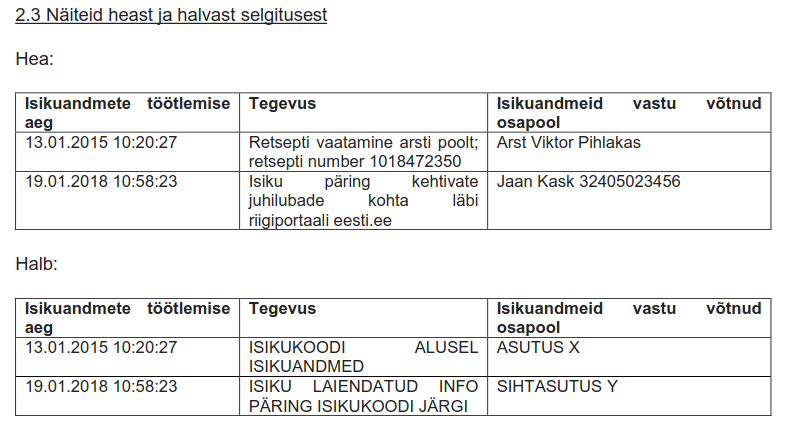
\includegraphics[width=450px]{english/figures/aj_good_and_bad_practices.png}

Apparently, the advice is often ignored.

Furthermore, currently there is no law requiring institutions to implement the Andmejälgija protocol, meaning that its use is pretty much voluntary.

In the following chapters I will cover different state databases and their implementations of Andmejälgija, and whether they implement the protocol at all.